% ================= 4 INITIAL RESULTS =================
\section{Initial results}

\begin{frame}{Where is the unsteadiness?}
  \only<1>{
  \begin{columns}[T]
    \column{.5\textwidth}\centering
    \begin{figure}
      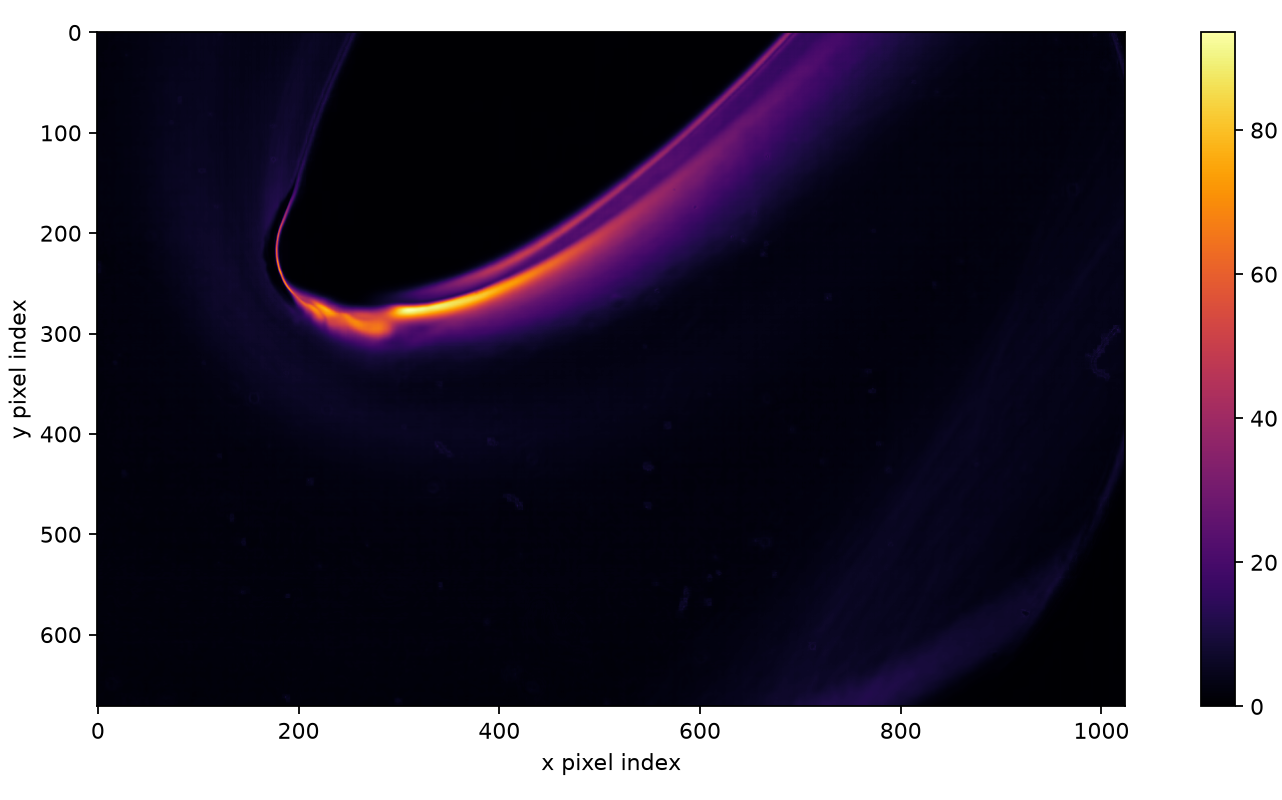
\includegraphics[width=6.85cm]{figures/run15_sd.png}
      \caption{S.D. of pixel intensity. Run 15 (Shot at 10,000 fps).}
    \end{figure}
    \column{.5\textwidth}\centering
    \begin{figure}
      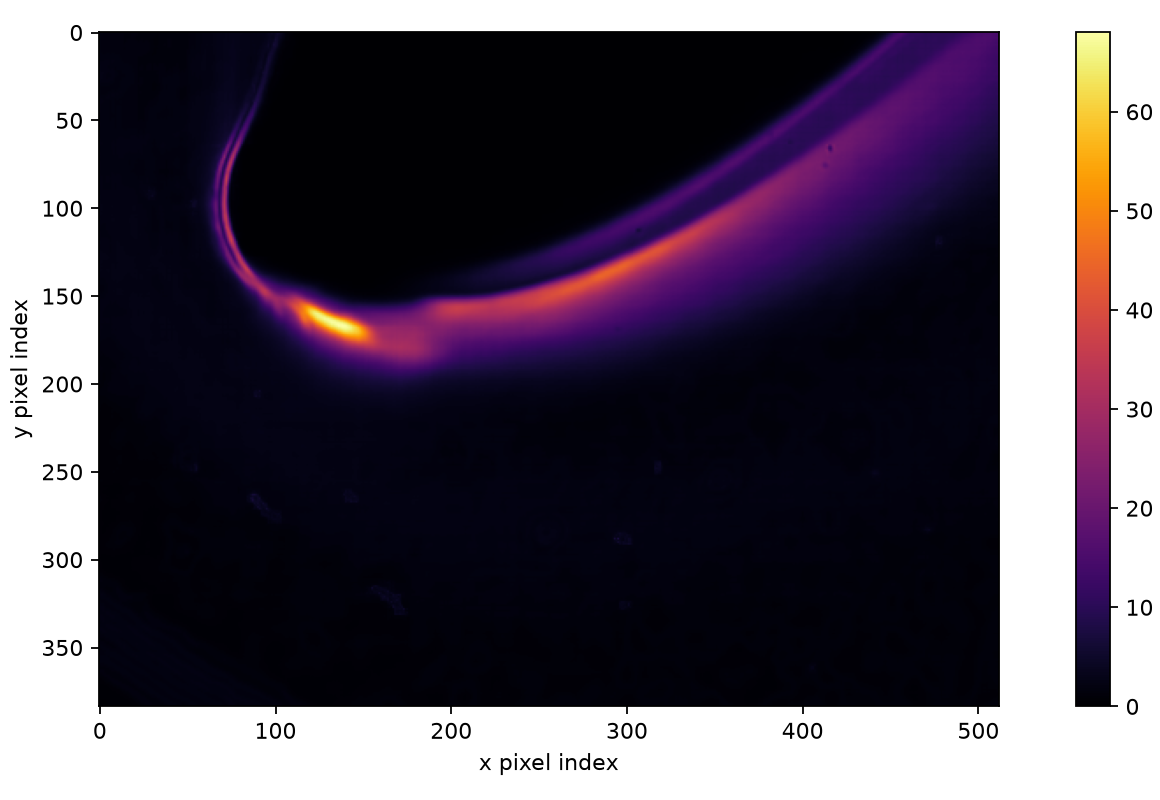
\includegraphics[width=6.2cm]{figures/run17_sd.png}
      \caption{S.D. of pixel intensity. Run 17 (Shot at 30,000 fps).}
    \end{figure}
  \end{columns}}
  \only<2->{
  \vspace{-1em}
  \begin{centering}
    \begin{figure}
      % \caption{Standard deviation of pixel intensity. Run 16 (Shot at 50,000 fps).}
      % \vspace{-1.5em}
      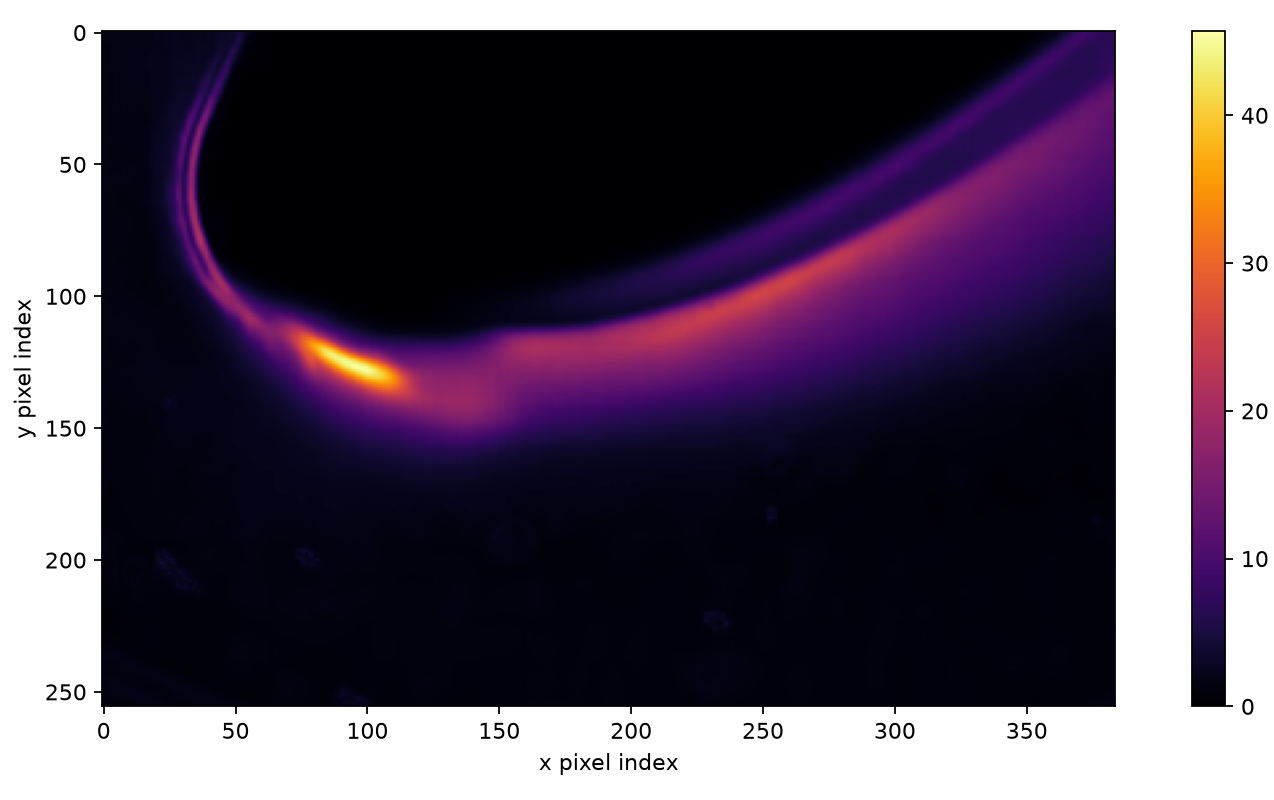
\includegraphics[width=0.7\textwidth]{figures/run16_sd.png}
    \end{figure}
  \end{centering}
  }\only<3->{\vspace{-0.8em}
  \begin{block}{\footnotesize Takeaway}\footnotesize Separate unsteadiness phenomenon at the shock from the downstream BL.\end{block}}
\end{frame}

\begin{frame}{Tracking features in time - shock}
  \begin{columns}[c]
    \column{.32\textwidth}\centering
    \begin{figure}
      % \caption{Standard deviation of pixel intensity. Run 16 (Shot at 50,000 fps).}
      % \vspace{-1.5em}
      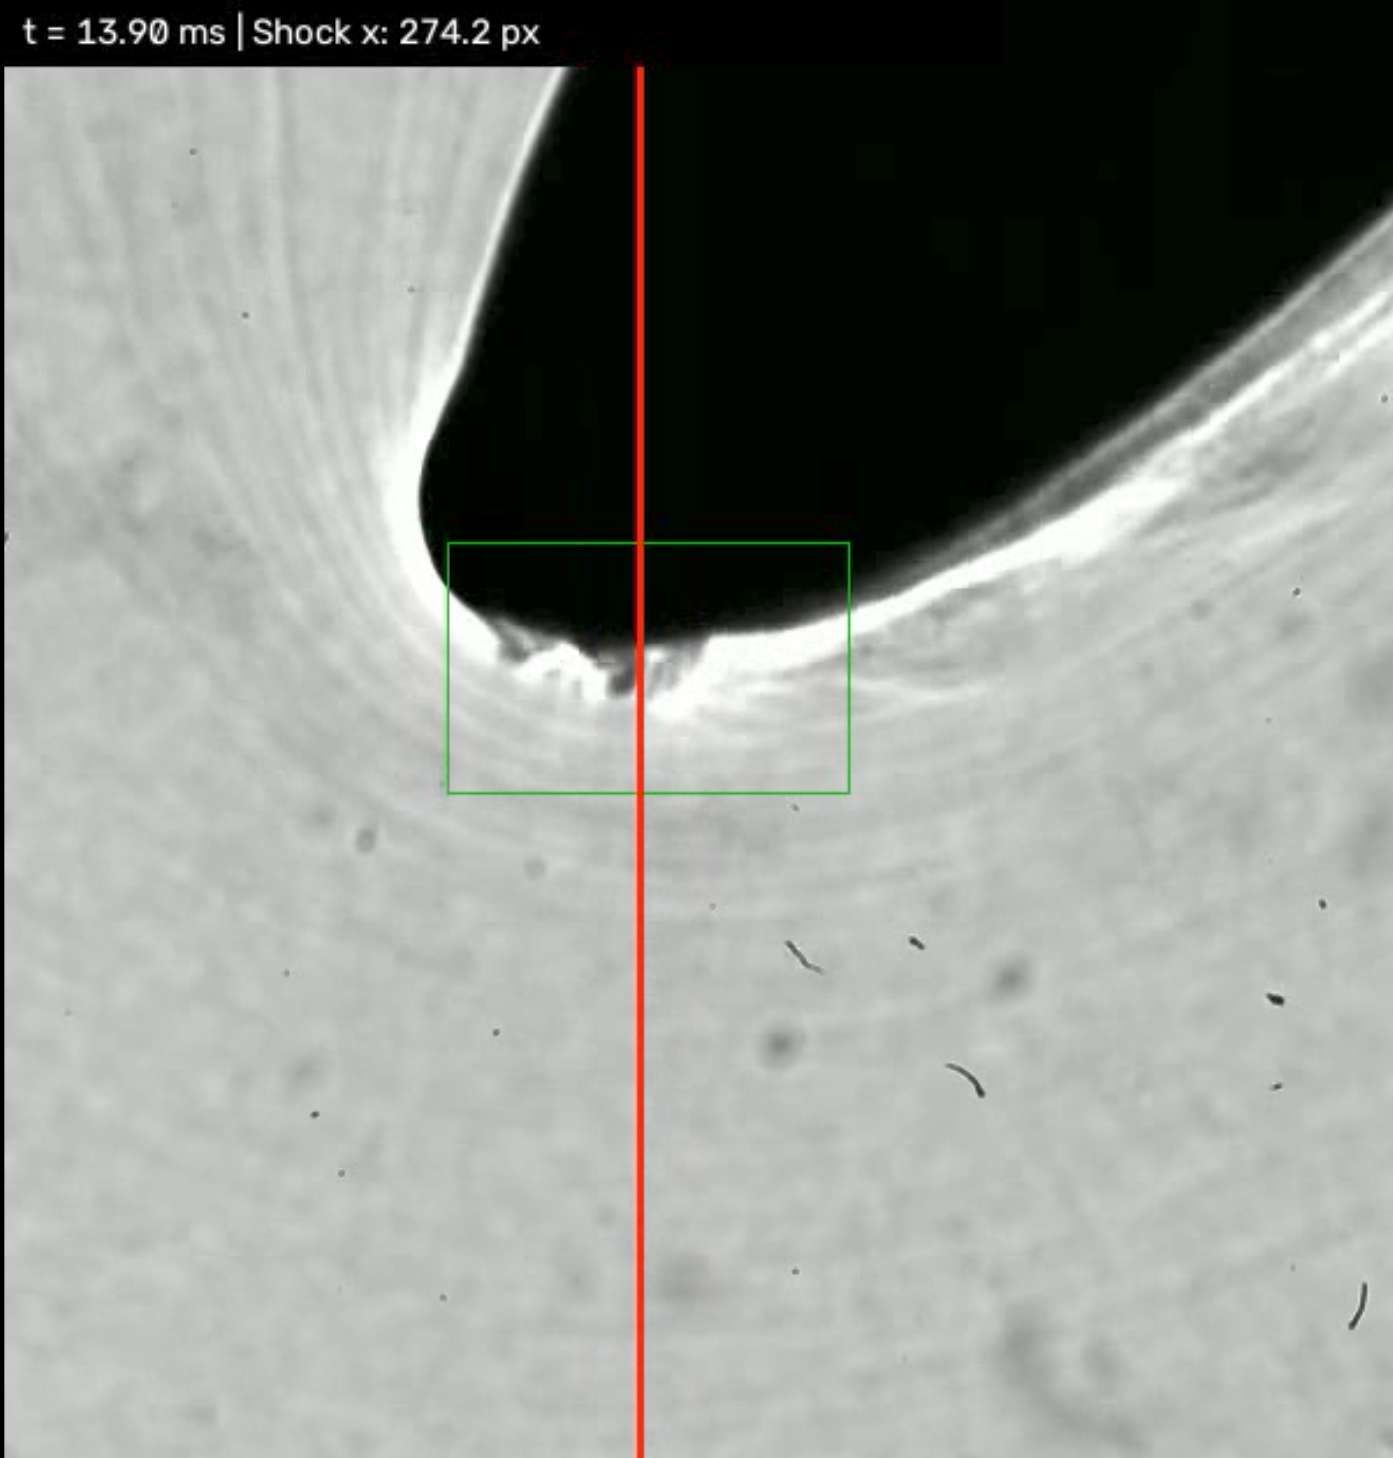
\includegraphics[width=\textwidth]{figures/shock_tracking_shadowgraph.png}
    \end{figure}
    \column{.68\textwidth}\centering
    \begin{figure}
      % \caption{Standard deviation of pixel intensity. Run 16 (Shot at 50,000 fps).}
      % \vspace{-1.5em}
      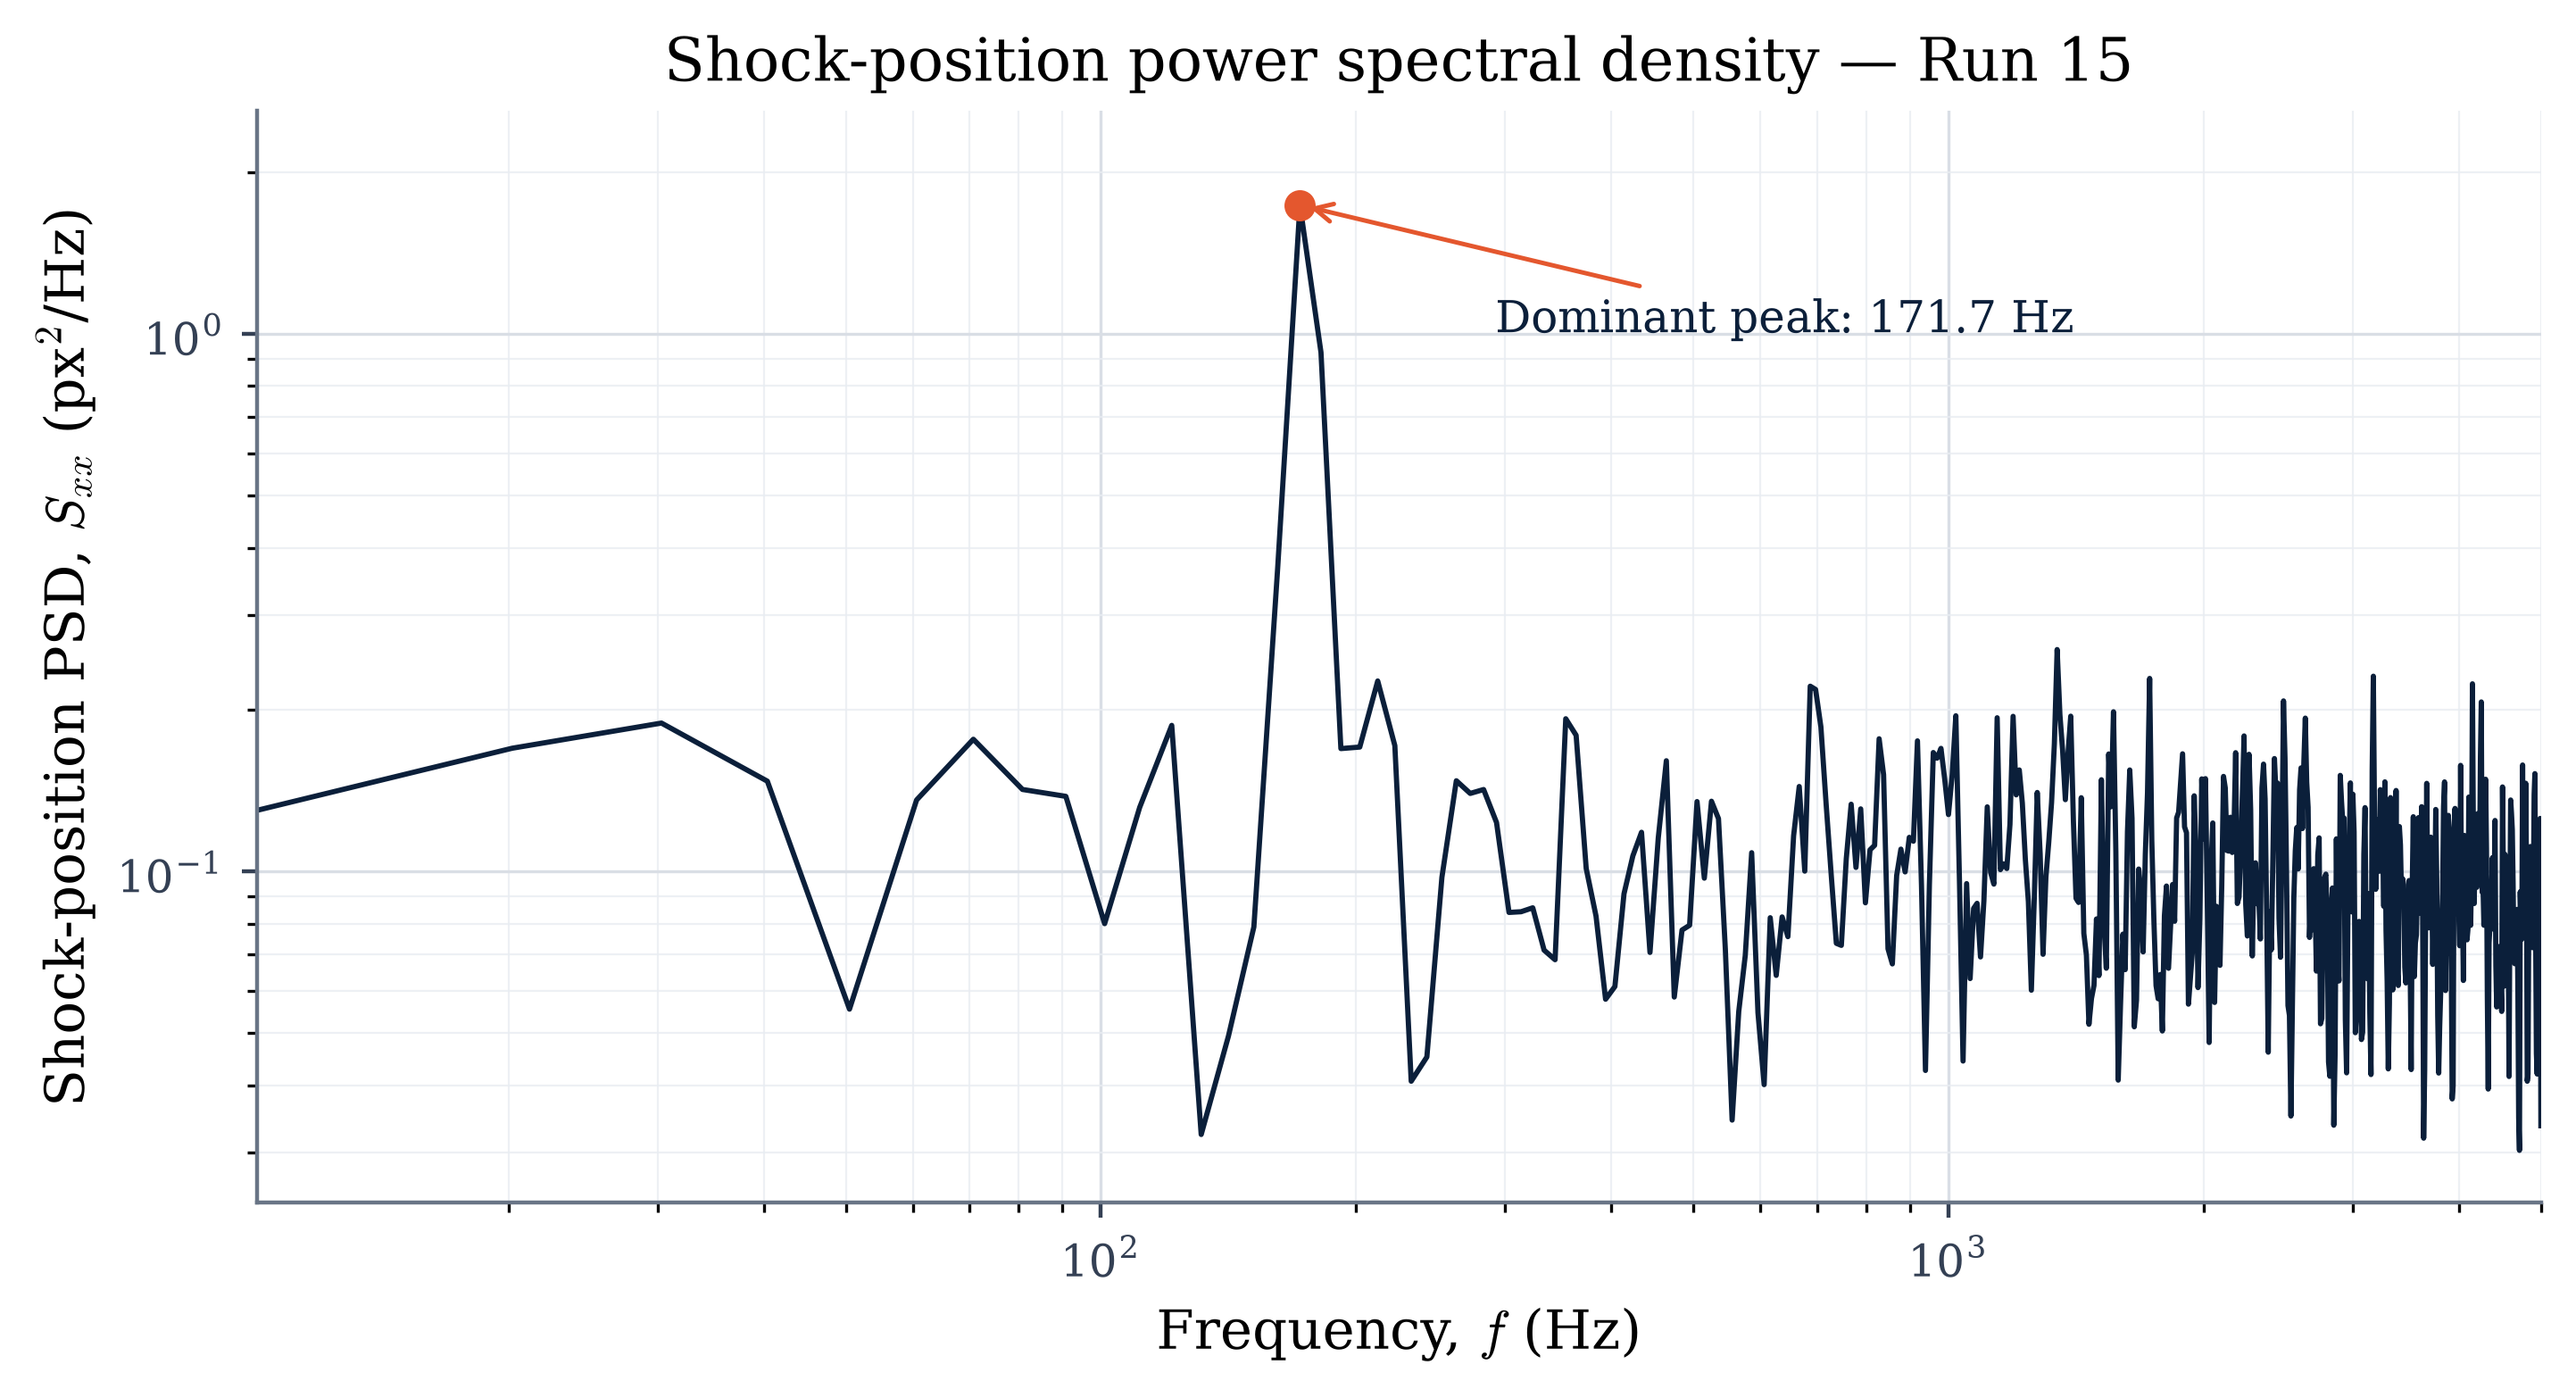
\includegraphics[width=\textwidth]{figures/shock_position_psd_run15.png}
    \end{figure}
  \end{columns}
  % \vspace{.2cm}
  % \begin{block}{Takeaway}\small [Dominant frequency, is it narrow or broadband, how many cycles recorded.]\end{block}
\end{frame}

\begin{frame}{Tracking features in time - boundary layer}
  \centering
  \only<1>{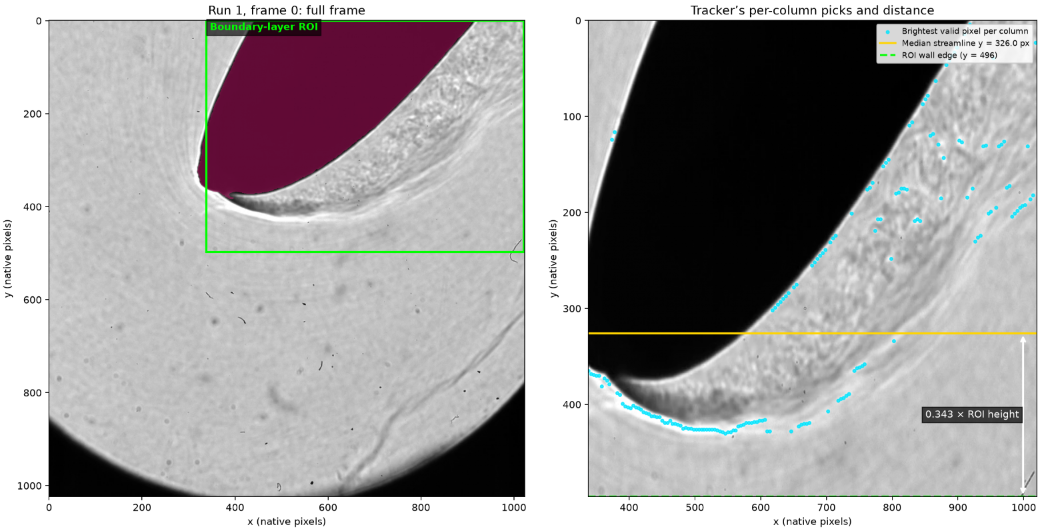
\includegraphics[width=0.9\textwidth]{figures/BL_tracking_shadowgraph.png}}
  \only<2>{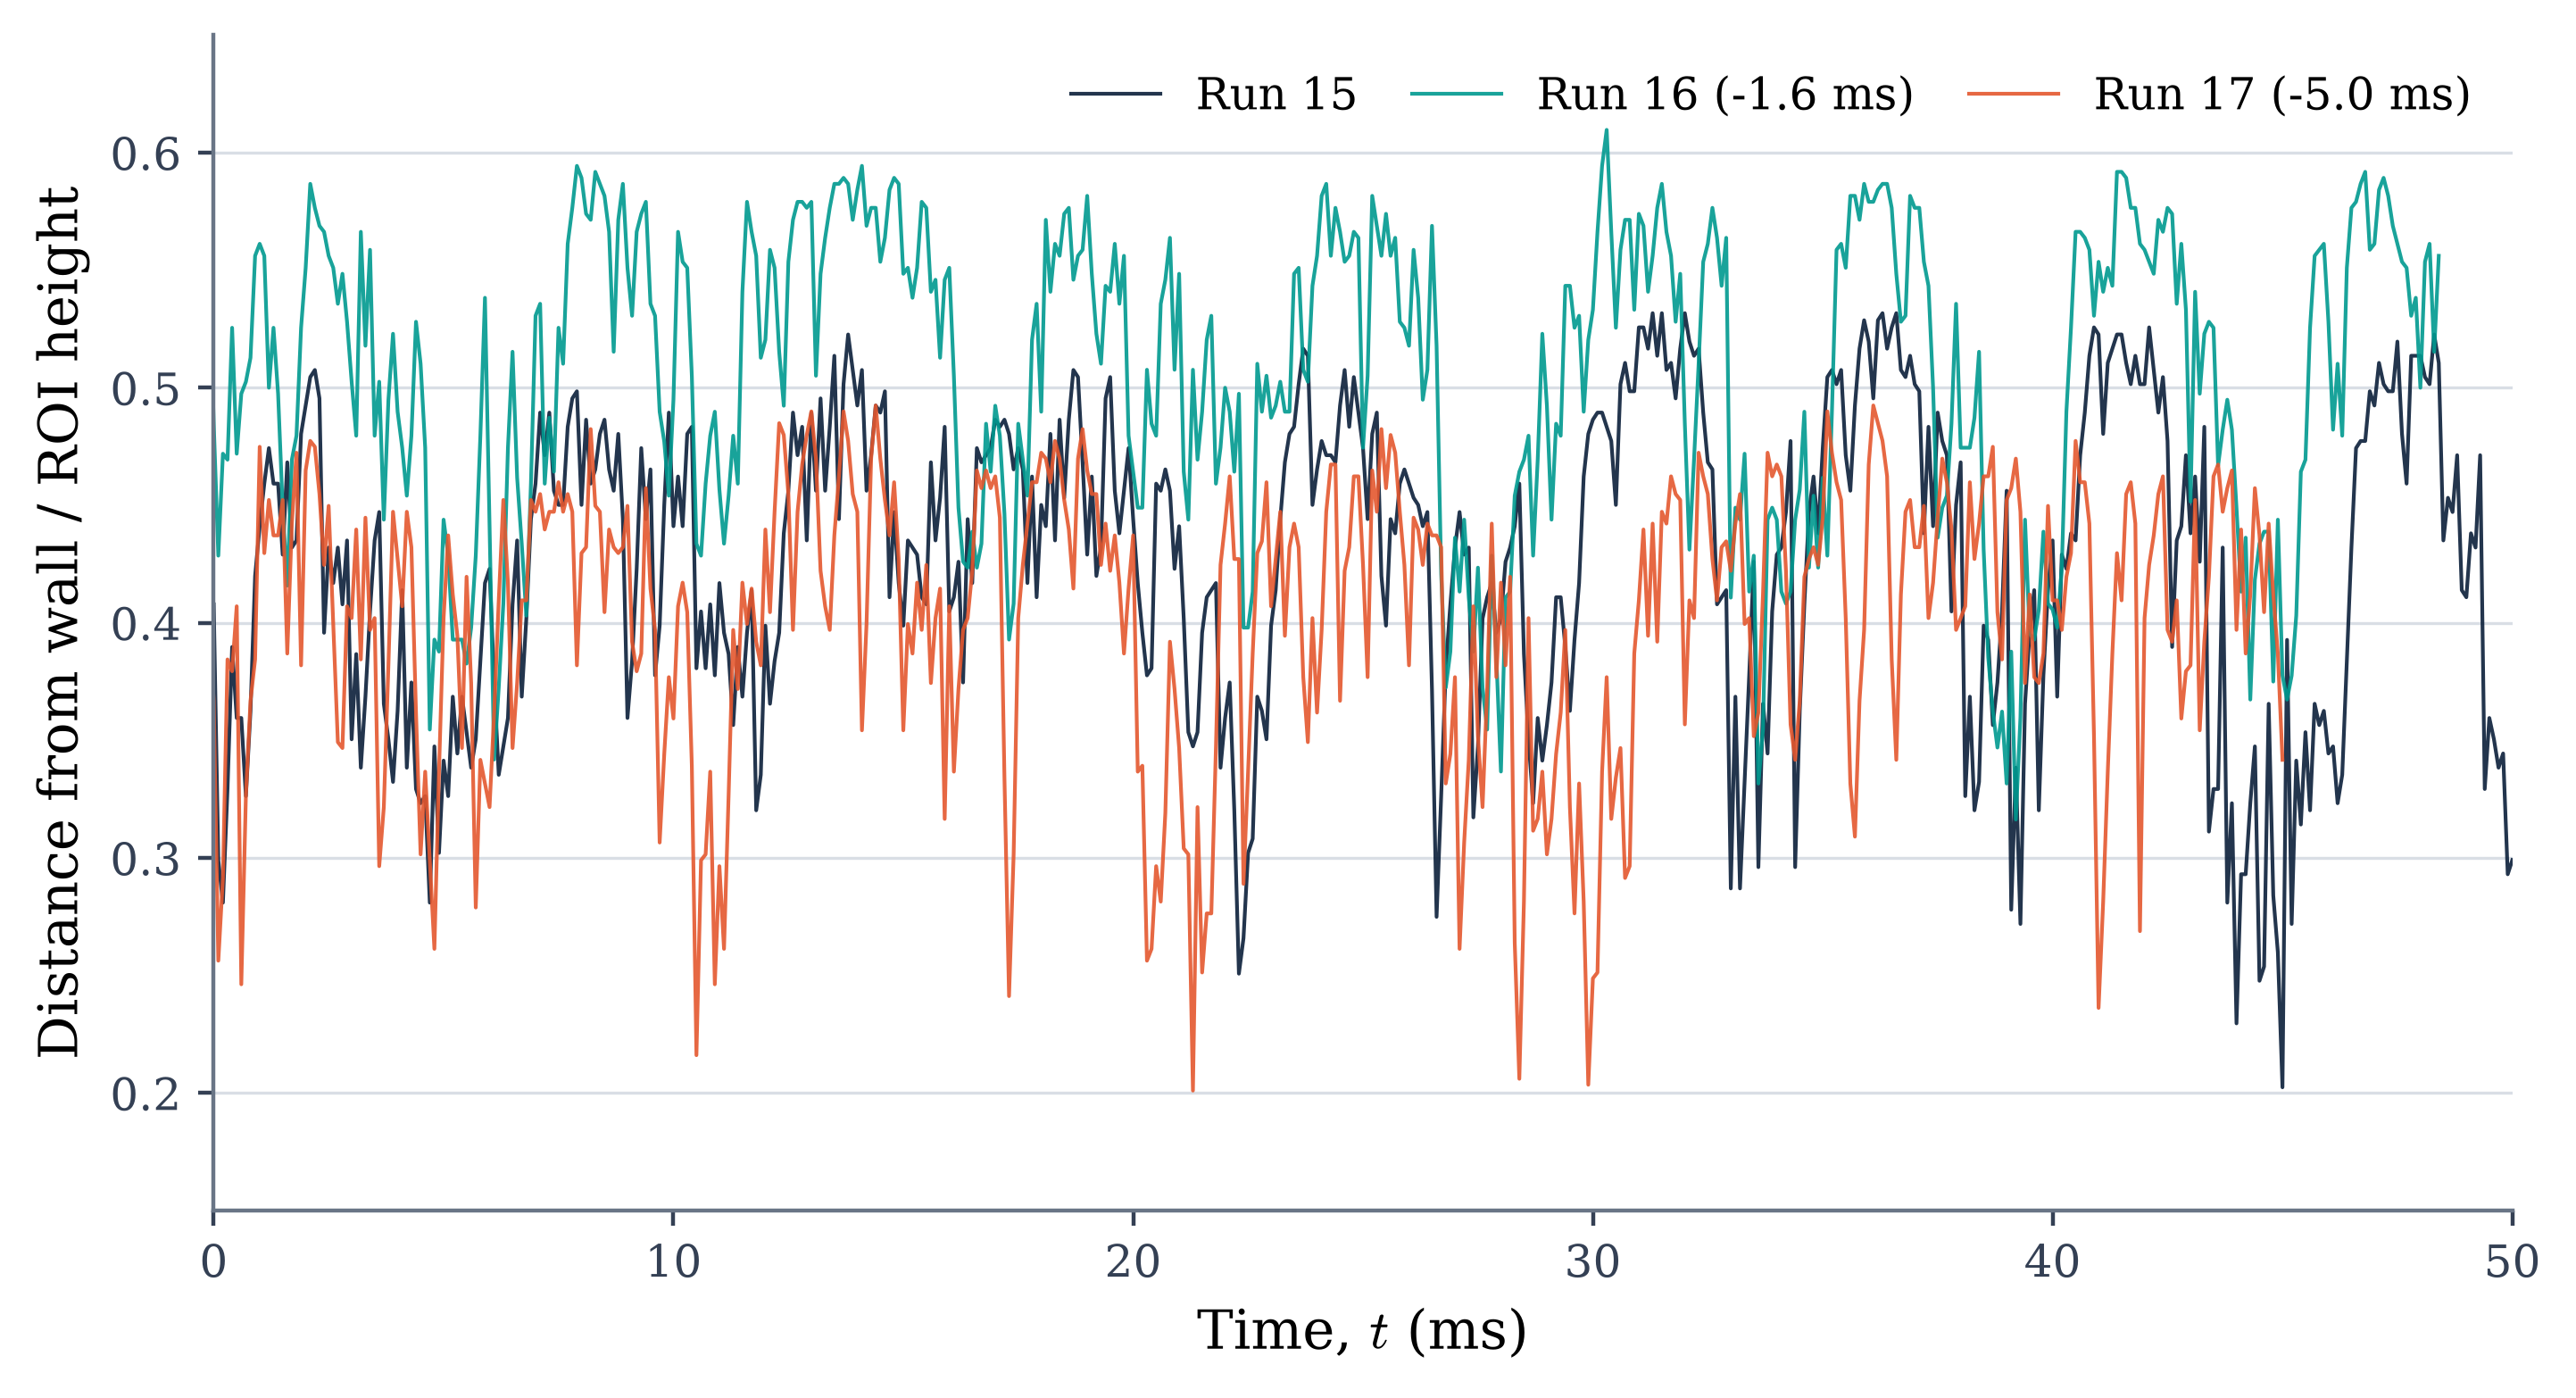
\includegraphics[width=0.9\textwidth]{figures/boundary_layer_motion_runs15-17.png}}
  \only<3>{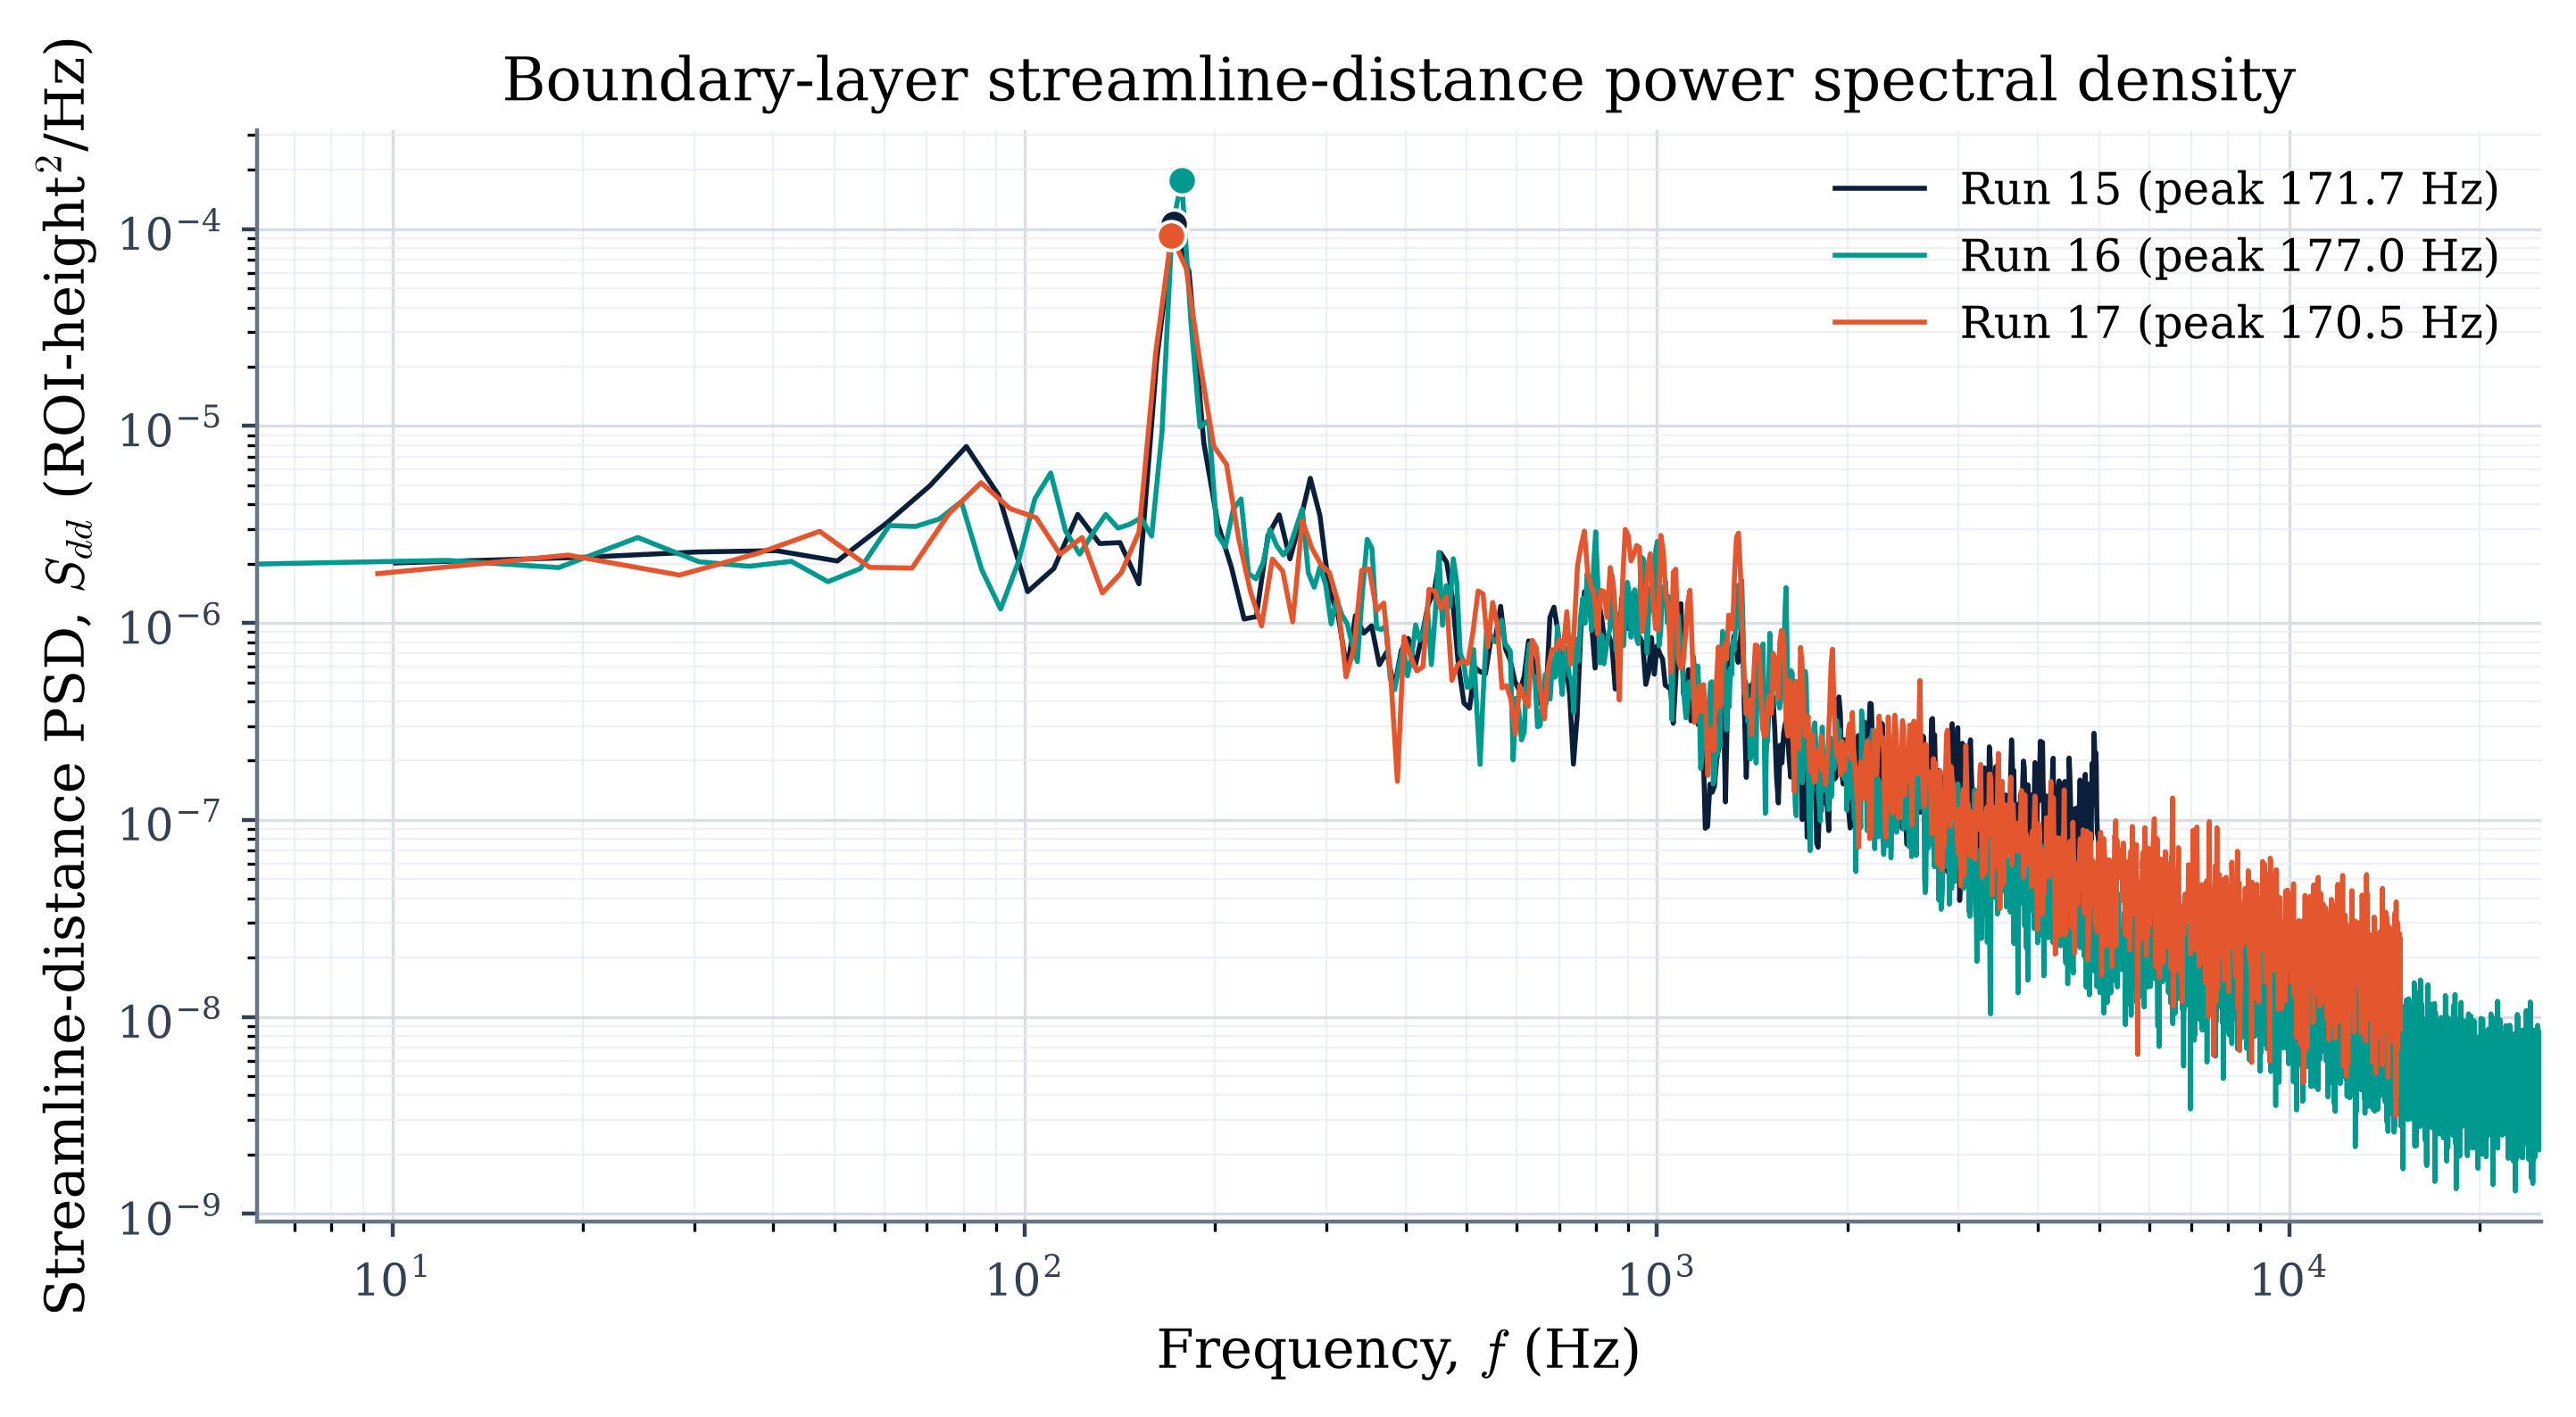
\includegraphics[width=0.9\textwidth]{figures/BL_psd.png}}
\end{frame}

\begin{frame}{Early lip-profile comparison}
  \centering
  {\small
  \begin{tabular}{@{}lccc@{}}\toprule
     & Thinner & Baseline & Thicker\\\midrule
    Critical $M_{\mathrm{entry}}$ & -- & 0.1575 & --\\
    Peak $M_{is}$ at onset & -- & 1.44 & --\\
    Dominant $f$ [Hz] & -- & $\sim$600 & --\\
    $St$ & -- & -- & --\\
    $\sigma_{x_s}/D$ & -- & -- & --\\
    Footprint $\Delta x_{\mathrm{foot}}/D$ & -- & -- & --\\\bottomrule
  \end{tabular}}\\[6pt]
  {\scriptsize\color{navy!60}Baseline values taken from the earlier thesis; fill in the rest as data are processed.}
\end{frame}
